\documentclass{standalone}
\usepackage{tikz}
\usetikzlibrary{shapes.geometric, arrows}

\usepackage[scaled]{helvet}
\usepackage[T1]{fontenc}
\renewcommand\familydefault{\sfdefault}

\tikzstyle{processnode} = [rectangle, rounded corners, 
minimum width=2cm, 
minimum height=1cm,
text width=1.8cm,
text centered, 
draw=black]

\tikzstyle{datanode} = [rectangle, thick,
fill=black!20,
minimum width=2cm, 
minimum height=1cm,
text width=1.7cm,
text centered, 
draw=black]

\tikzstyle{invisible} = [
minimum width=2cm, 
minimum height=1cm,
text width=2cm,
text centered]

\tikzstyle{io} = [trapezium, 
trapezium stretches=true, % A later addition
trapezium left angle=70, 
trapezium right angle=110, 
minimum width=3cm, 
minimum height=1cm, text centered, 
draw=black, fill=blue!30]

\tikzstyle{process} = [rectangle, 
minimum width=3cm, 
minimum height=1cm, 
text centered, 
text width=3cm, 
draw=black, 
fill=orange!30]

\tikzstyle{decision} = [diamond, 
minimum width=3cm, 
minimum height=1cm, 
text centered, 
draw=black, 
fill=green!30]
\tikzstyle{arrow} = [thick,->,>=stealth]
\begin{document}

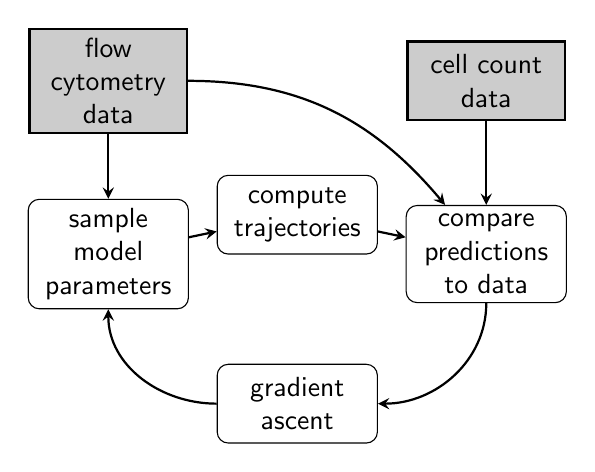
\begin{tikzpicture}[node distance=1.2cm]

\node (flow) [datanode] {flow cytometry data};

\node (sample) [processnode, below of=flow, yshift=-1cm] {sample model parameters};

\node (traj) [processnode, right of=sample, xshift=1.2cm, yshift=0.5cm] {compute trajectories};

\node (loss) [processnode, right of=traj, xshift=1.2cm, yshift=-0.5cm] {compare predictions to data};

\node (count) [datanode, thick, above of=loss, yshift=1cm] {cell count data};

\node (grad) [processnode, below of=traj, yshift=-1.2cm] {gradient ascent};


\draw [arrow] (flow) -- (sample);

\draw [arrow] (flow) to [out=0, in=130] (loss);

\draw [arrow] (count) -- (loss);

\draw [arrow] (sample) -- (traj);

\draw [arrow] (traj) -- (loss);

\draw [arrow] (loss) to [out=-90, in=0] (grad);

\draw [arrow] (grad) to [out=180, in=-90] (sample);





\end{tikzpicture}
\end{document}